\section{Measurement of the antitriton inelastic cross section}\label{sec:ResTritonSigmaInel}
\subsection{Physics motivation and overview of the analysis method}
The measurement of \sigmainelH\ does not have the same astrophysical motivation as the measurement of \sigmainel\ , since \atrit\ is an unstable nucleus with a half-life of $\approx 12.3$ years. Instead, the main motivation for this measurement is the comparison to the \ahe\ inelastic cross section. This could shine light on any isospin dependence of the annihilation probability of antinuclei. Such an effect might also elucidate how the strong force interacts with isospin, in a potentially more sensitive way than observing neutrons, since they are much harder to detect due to not being charged. And while the current statistical uncertainties are unable to resolve any difference, the two measurements provide a proof of concept that this dependence can be measured by means of comparing the inelastic cross sections of $A=3$ antinuclei.
\subsection{Feasibility of the momentum range}
\begin{figure}
    \centering
    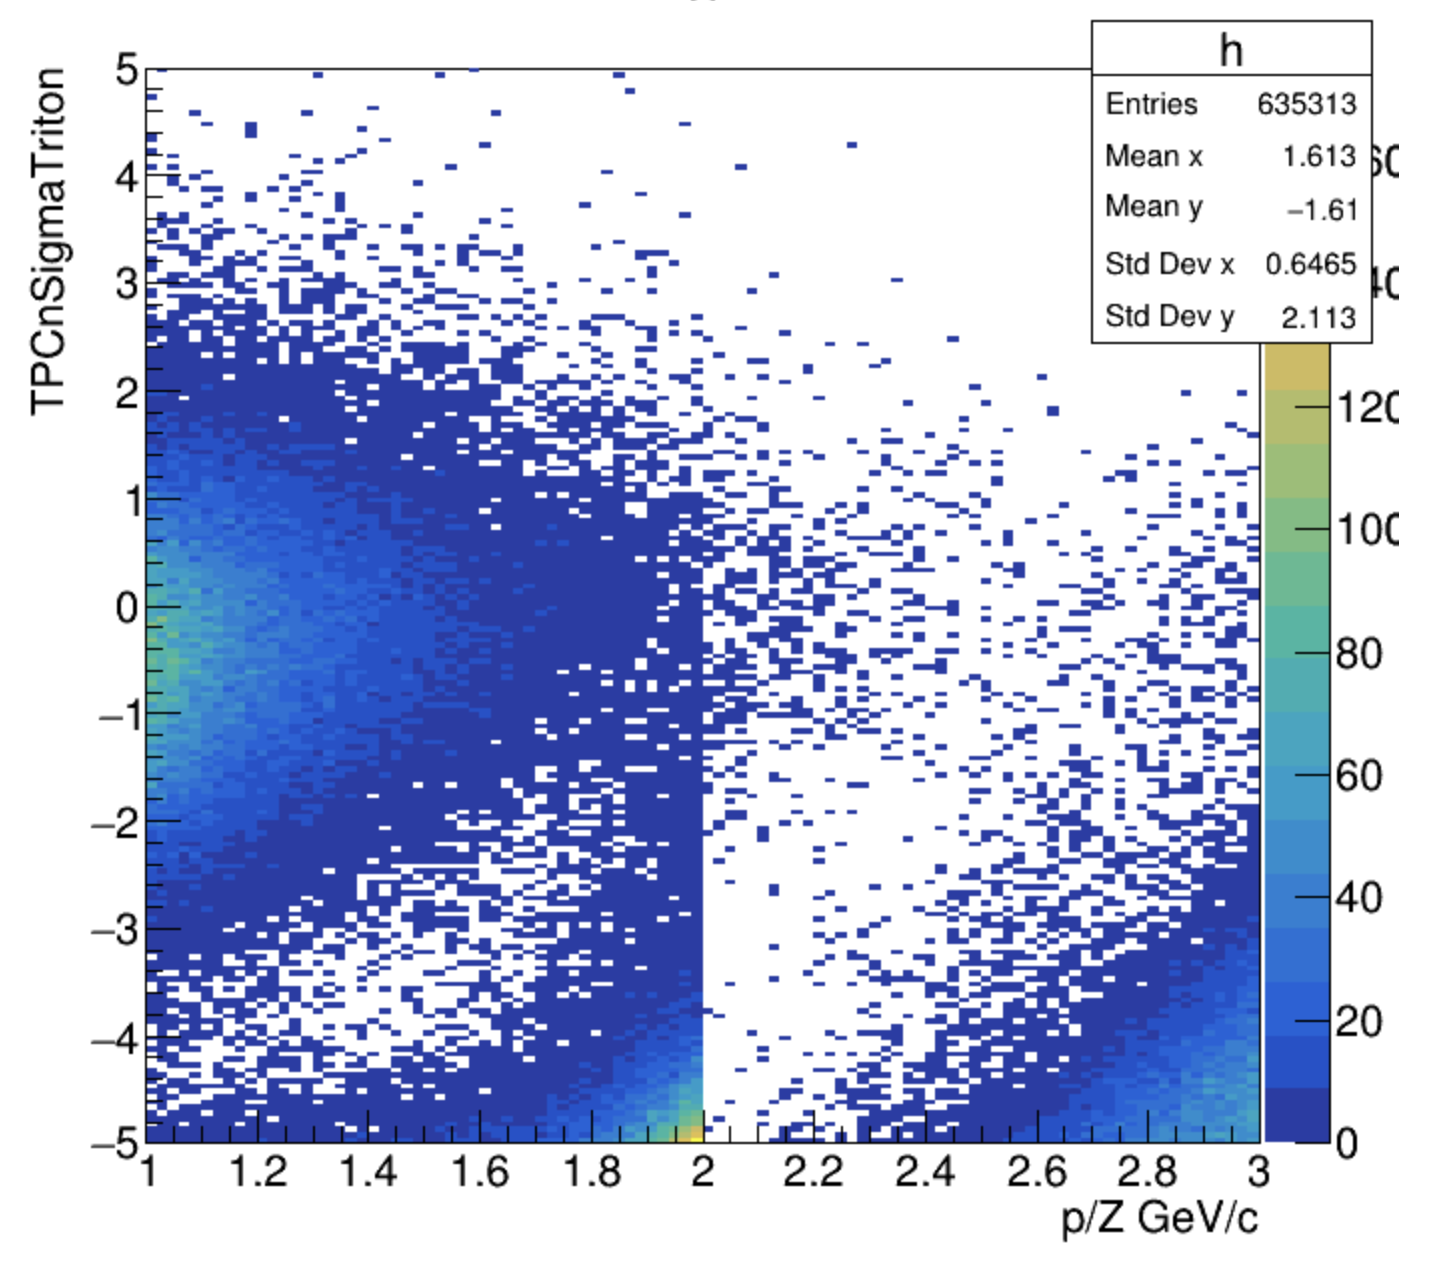
\includegraphics[width=0.48\textwidth]{figures/triton/tbar_TPCnSigma_noTOF_noDCA.png}
    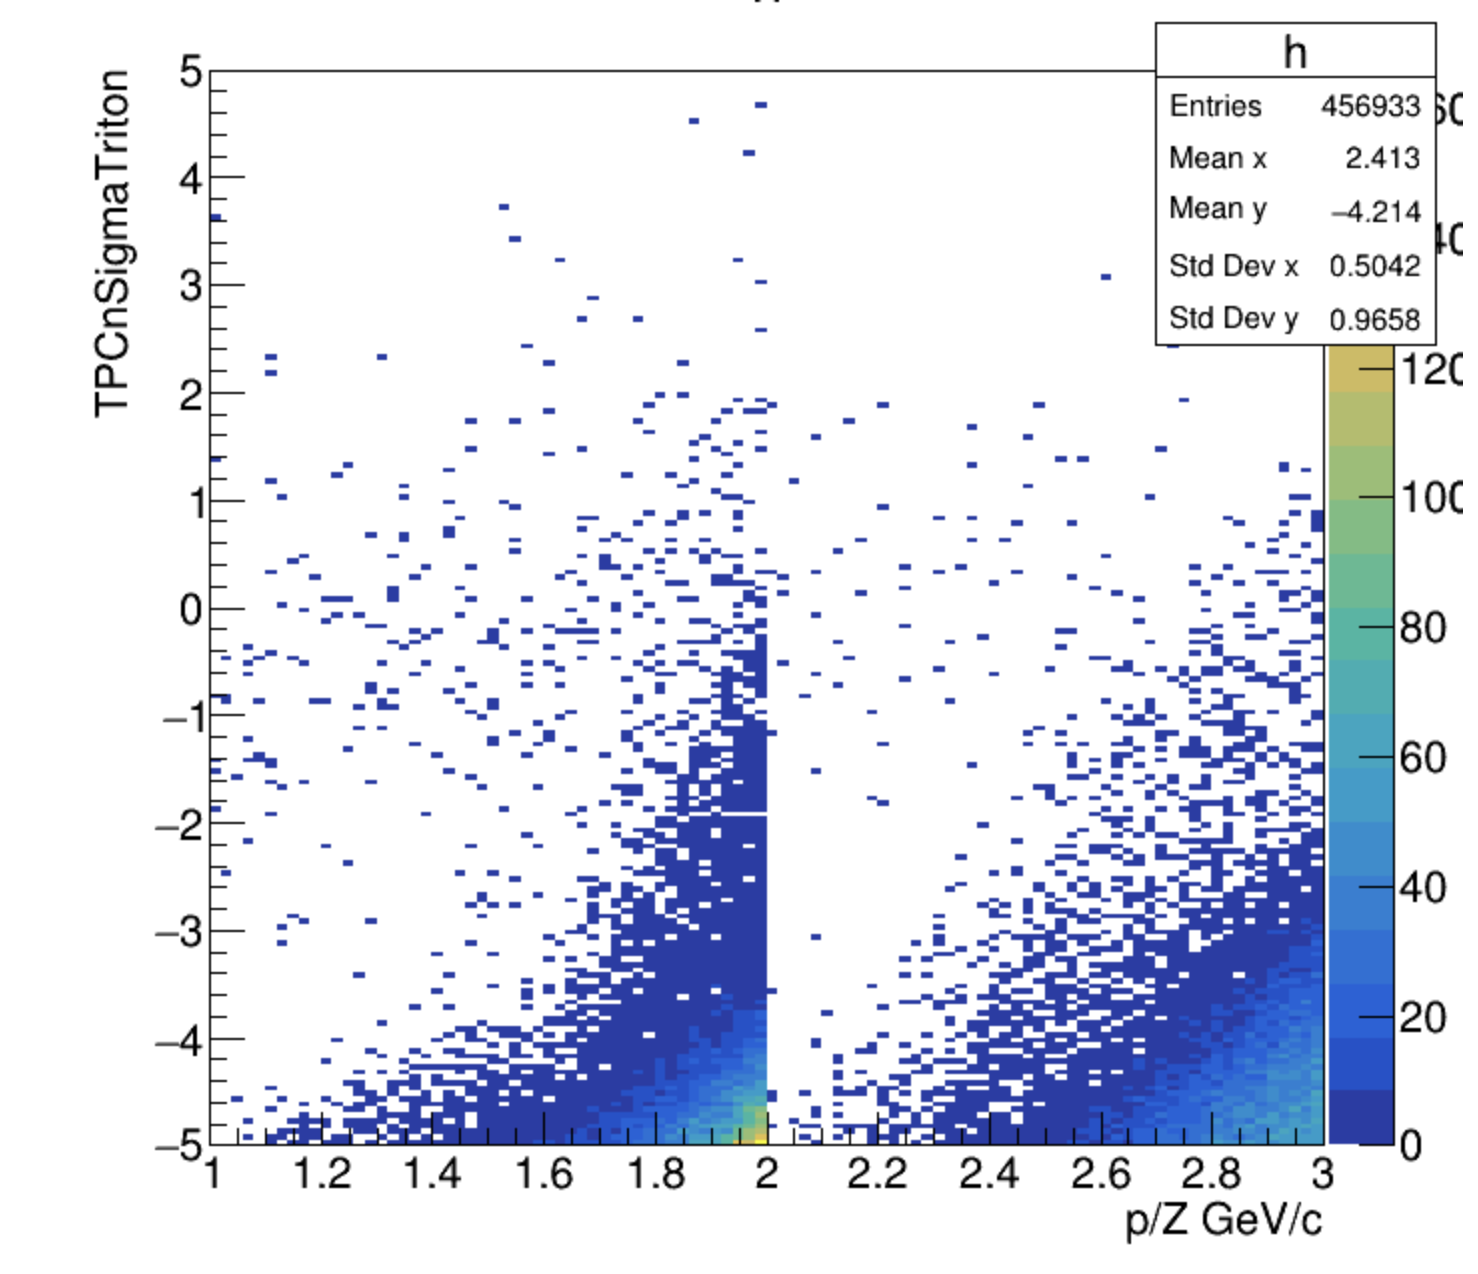
\includegraphics[width=0.48\textwidth]{figures/triton/tbar_TPCnSigma_noTOFcut.png}
    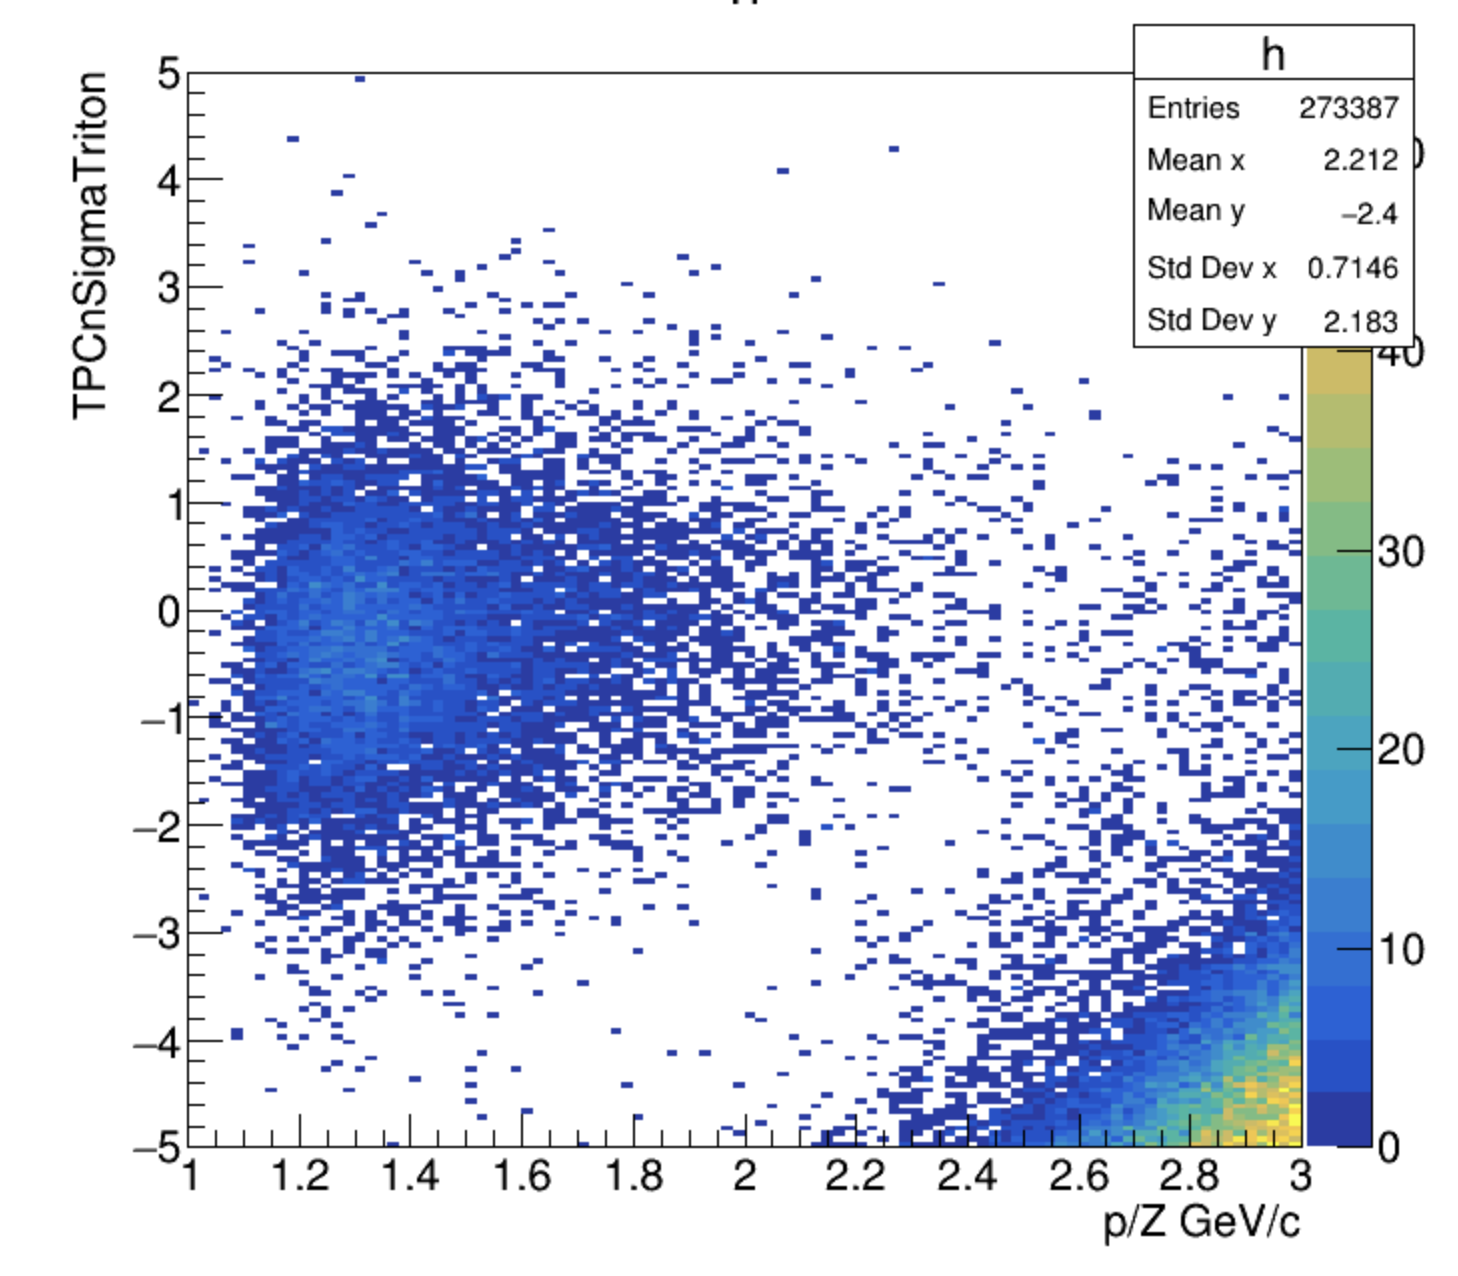
\includegraphics[width=0.48\textwidth]{figures/triton/tbar_TPCnSigma_TOF_cit_noDCA_cut.png}
    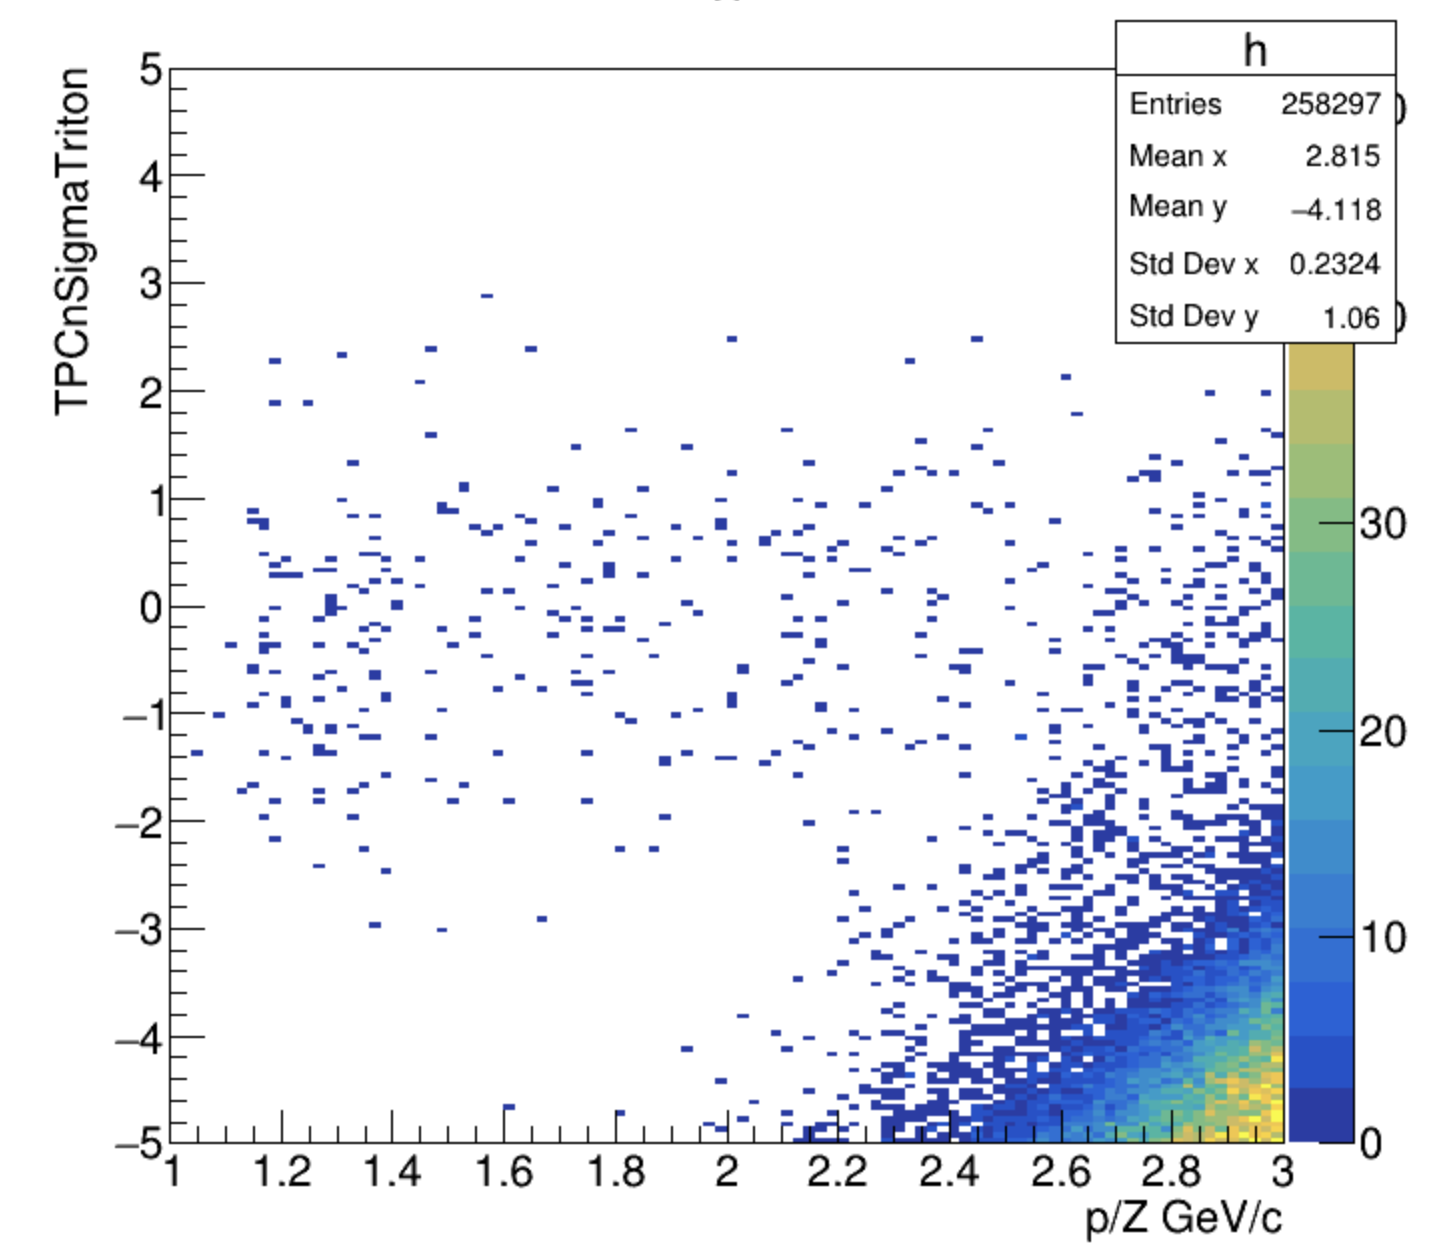
\includegraphics[width=0.48\textwidth]{figures/triton/tbar_TPCnSigma_TOF_cut_and_DCA_cut.png}
    \caption{$n\sigma_{\mathrm{TPC}}$ vs momentum plots for tritons. A cut on the $m_{\mathrm{TOF}}$ is applied below 2 GeV/$c$ in all figures. (Top left) the original distribution without an additional cut on either DCA or $m_{\mathrm{TOF}}$. (Top right) the distribution after a cut of $|\mathrm{DCA}_{xy}|<1\ mm\ \textrm{and}\  |\mathrm{DCA}_z|<1\ mm$ is applied. (Bottom left) the distribution after the cut on $m_{\mathrm{TOF}}$ is extended to momenta as low as 1 GeV/$c$. (Bottom left) the distribution after both the DCA and $m_{\mathrm{TOF}}$ cuts were applied.}
    \label{fig:Tritons_momentum_range}
\end{figure}
Due to the single charge of \atrit\ , there are a few noteworthy differences in the particle identification in comparison to \ahe\ . The first and most important difference is that it is not clearly identifiable in the TPC alone at high momenta. The considerations for the identification are shown in figure \ref{fig:Tritons_momentum_range}, which shows how the TOF cut is able to remove the contamination up to a momentum of $\approx$ 2.4 GeV/$c$, while the DCA cut removes much of the secondary contribution at low momentum. Additionally, by comparing the top and bottom panels on the right side of figure \ref{fig:Tritons_momentum_range}, which show the effect of the TOF cut after the DCA cut is applied, we can see that the additional requirement of the TOF removes all the contamination at low momentum, while removing very little of the signal. This is compounded by the fact that by requiring the TOF, the particles have to traverse more material, and thus the ratio becomes more sensitive to the inelastic cross section. Thus, the TOF is used in the whole momentum range for the measurement of the \atrit\ /$^3\mathrm{H}$ ratio. 


\subsection{Secondary correction}
\begin{figure}
    \centering
    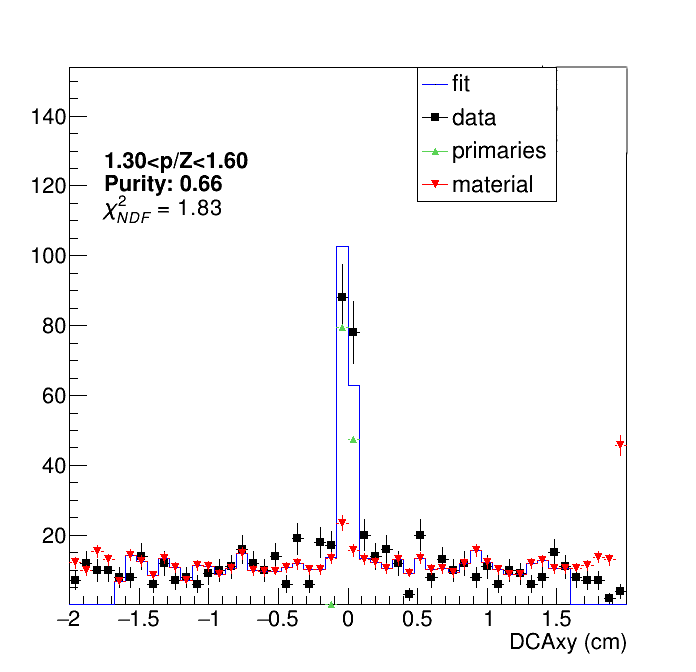
\includegraphics[width=0.32\textwidth]{figures/triton/Templates/TemplateFitHe3_1.3<p<1.6_rebin_2_Bin_1.png}
    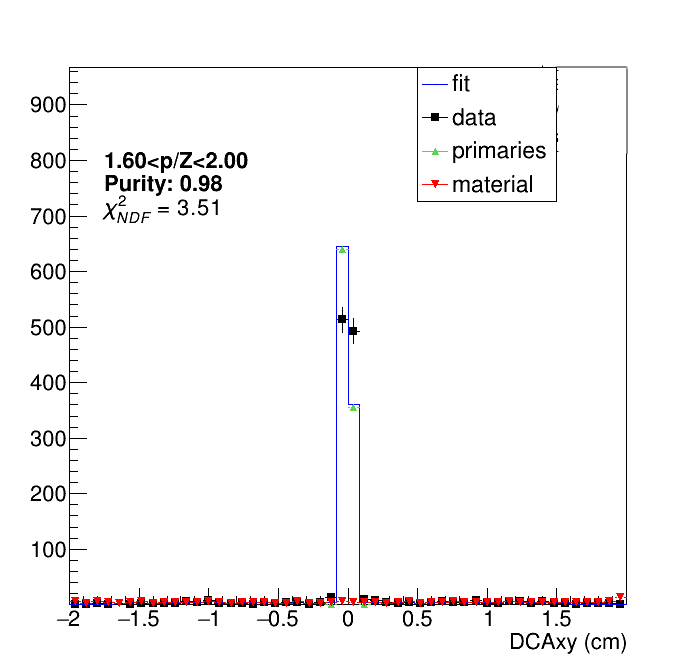
\includegraphics[width=0.32\textwidth]{figures/triton/Templates/TemplateFitHe3_1.6<p<2_rebin_2_Bin_2.png}
    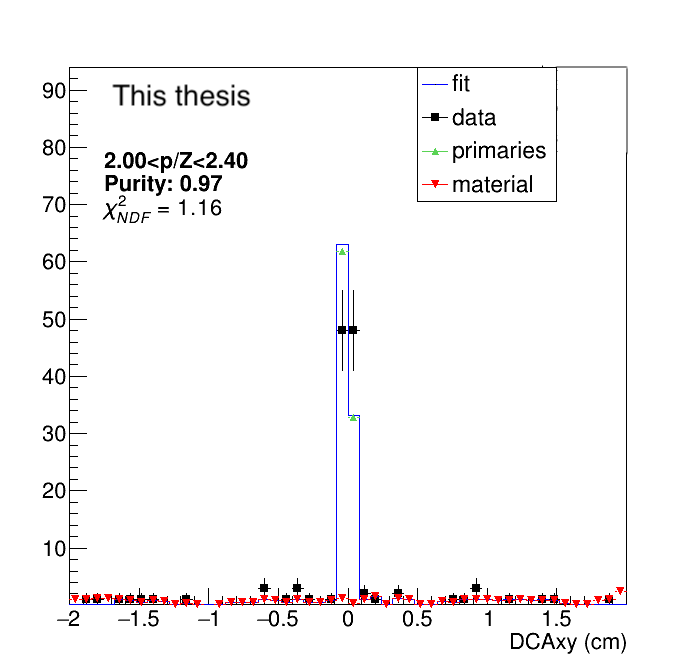
\includegraphics[width=0.32\textwidth]{figures/triton/Templates/TemplateFitHe3_2<p<2.4_rebin_2_Bin_3.png}
    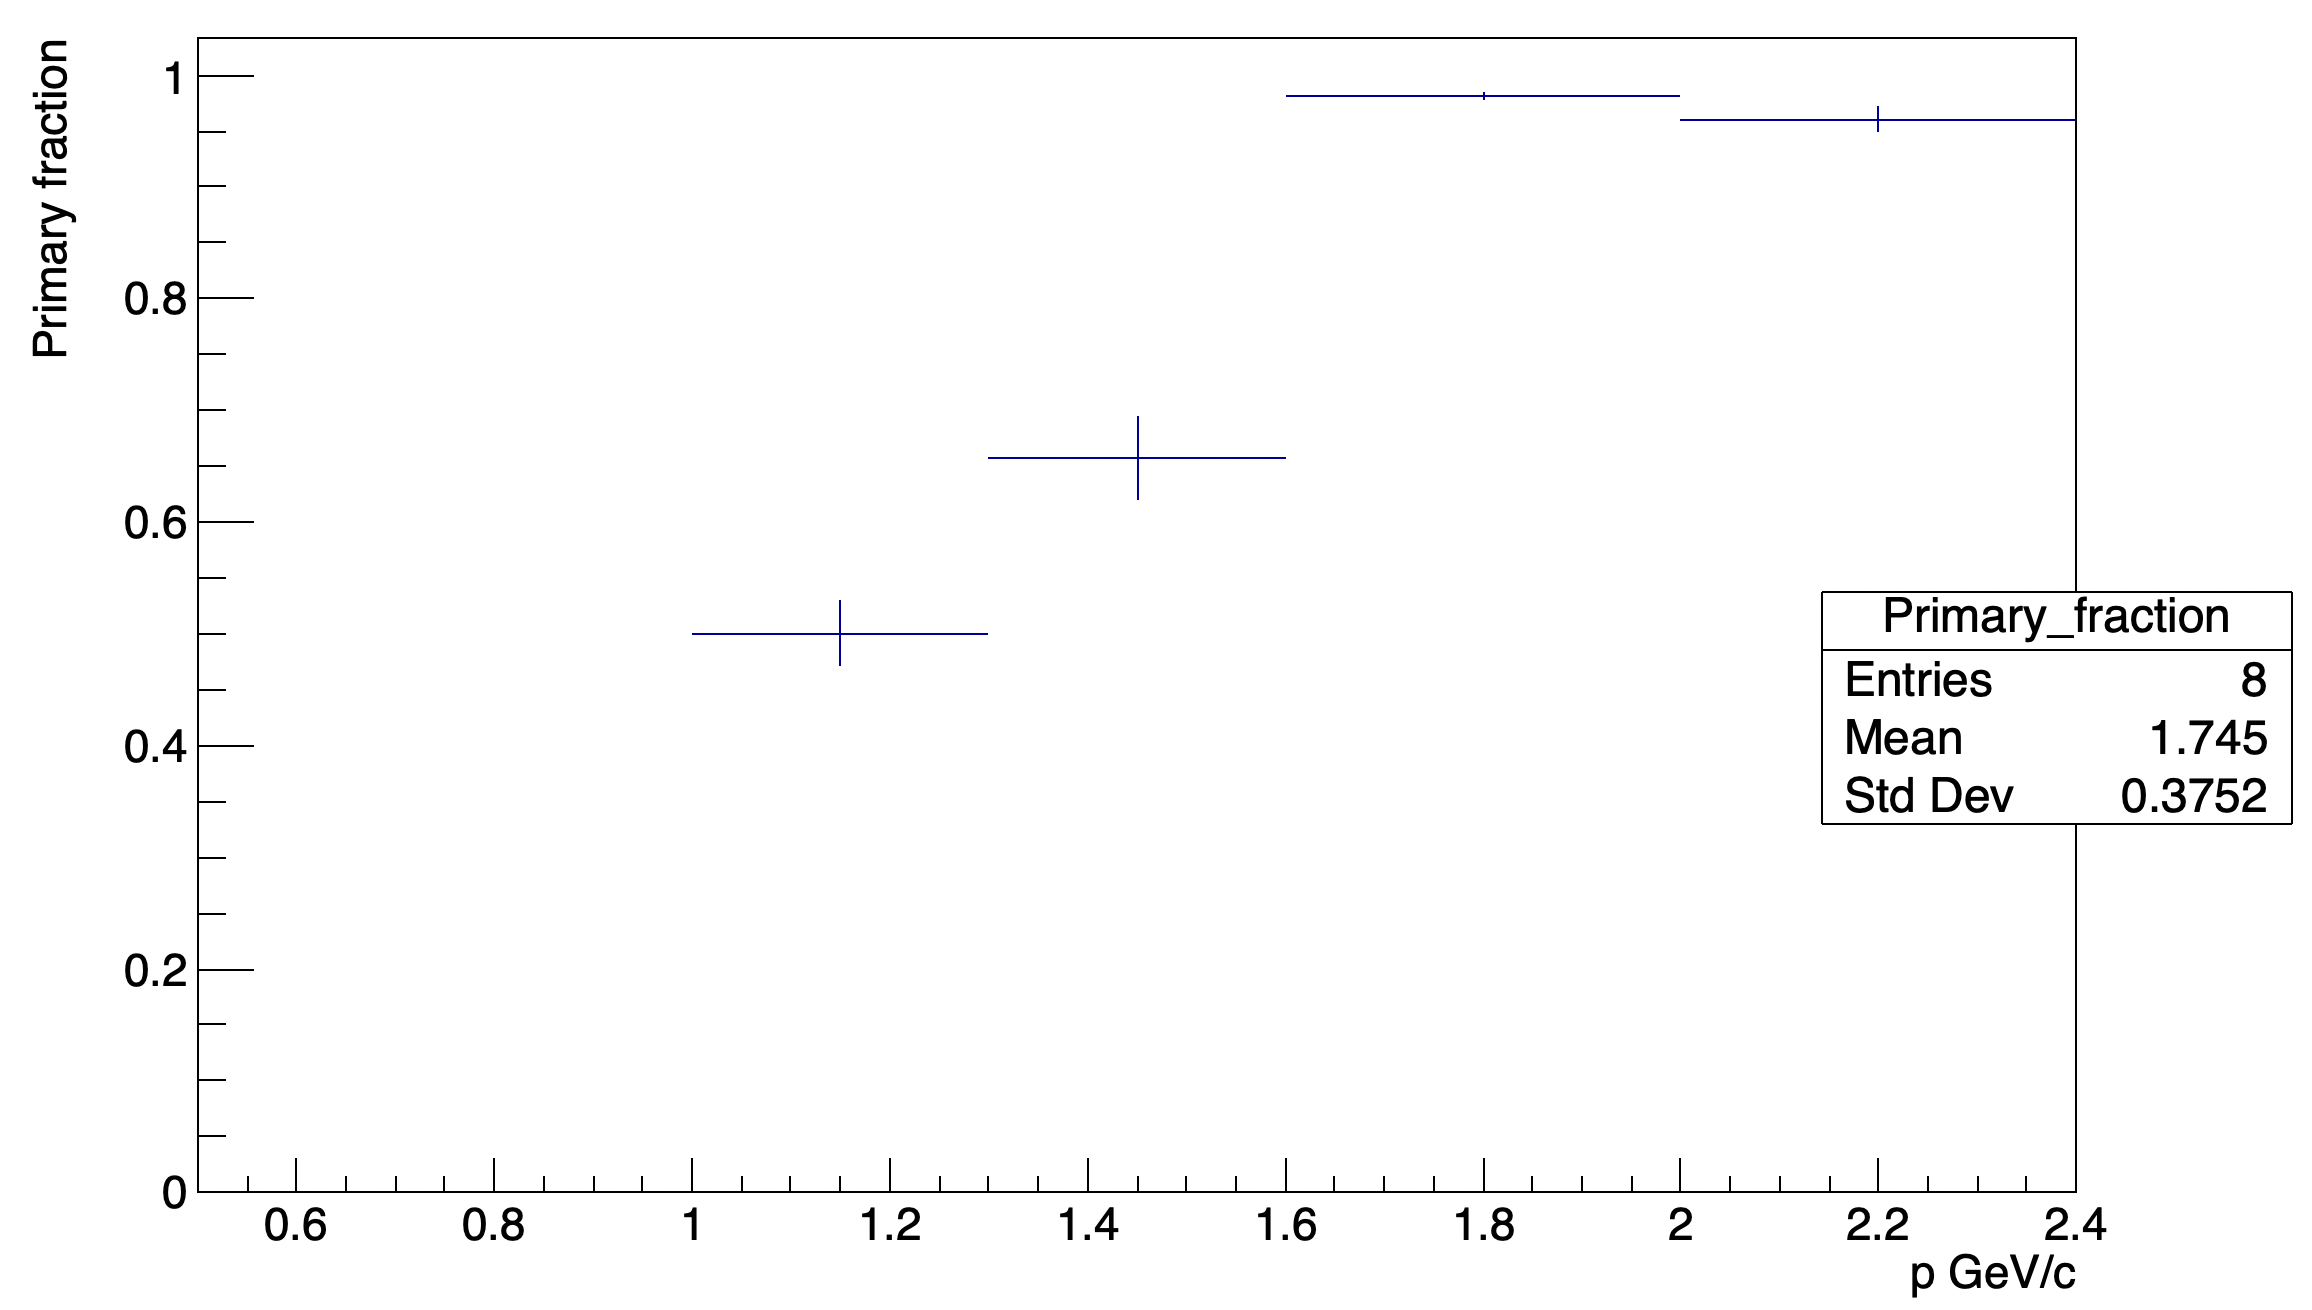
\includegraphics[width=0.75\textwidth]{figures/triton/tbar_Primary_fraction.png}
    \caption{(Top row) Template fits to the DCA distribution of $^3\mathrm{H}$, to account for the contributions from secondary nuclei from spallation processes. The primary fraction is evaluated as $f_p = \int_{-0.1cm}^{0.1cm} \mathrm{fit}_{\mathrm{signal}} d\mathrm{DCA} / \int_{-0.1cm}^{0.1cm}\ \mathrm{data}\ d\mathrm{DCA}$. The results are shown for each momentum bin. (Bottom row) The resulting primary fraction of $^3\mathrm{H}$ in pp collisions at $\sqrt{s}=13$ TeV.}
    \label{fig:TemplateFitsTriton}
\end{figure}
Similarly as for \ahe\ , the \atrit\ /$^3\mathrm{H}$ ratio still needs to be corrected for the remaining secondary nuclei from material spallation. This is done using template fits, according to the method described in \ref{sec:Meth:secondaryCorr}. The fits are shown in figure \ref{fig:TemplateFitsTriton}. It can be seen that the contribution is negligible in the second and third bin. In the first bin, the contribution from secondaries is well constrained. The resulting primary fraction is shown in the bottom of the figure. The uncertainty of the primary fraction is added to the systematic uncertainties on the \atrit\ /$^3\mathrm{H}$ ratio in quadrature.


\subsection{Results}
In this section, the measurements of \sigmainelH\ are presented. The left side of figure \ref{fig:Results:tbar:ratios} shows the \atrit\ /$^3\mathrm{H}$ ratio as measured in pp collisions, and the left side of figure \ref{fig:Results:tbar:xs} shows the resulting inelastic cross section measurement on the right. The measurement is consistent with the parameterization of used in Geant4 within a significance of 2 $\sigma$, but shows a hint at a systematically larger vale for \sigmainelH\ . The right side of figure \ref{fig:Results:tbar:ratios} shows the TOF/TPC ratio of \atrit\ in Pb -- Pb collisions at $\sqrt{s}=5.02$ TeV\footnote{These were not obtained by me or as part of this thesis, but were obtained for the same publication as the cross section in pp collisions.} and the corresponding measurement of \sigmainelH\ is shown in figure \ref{fig:Results:tbar:xs}. The measurements are compared with the results for \ahe\ in the left panel of figure \ref{fig:Results:tbar:xs}, all scaled to the same average material, which shows that the results for \atrit\ and \ahe\ are consistent within uncertainties. This means that within the current uncertainties, the annihilation cross sections are consistent with isospin symmetry. Improvements on the statistical precision of these measurements will help constrain this assumption further during the upcoming Run 3 and Run 4 data taking campaigns at the LHC. 

\begin{figure}
    \centering
    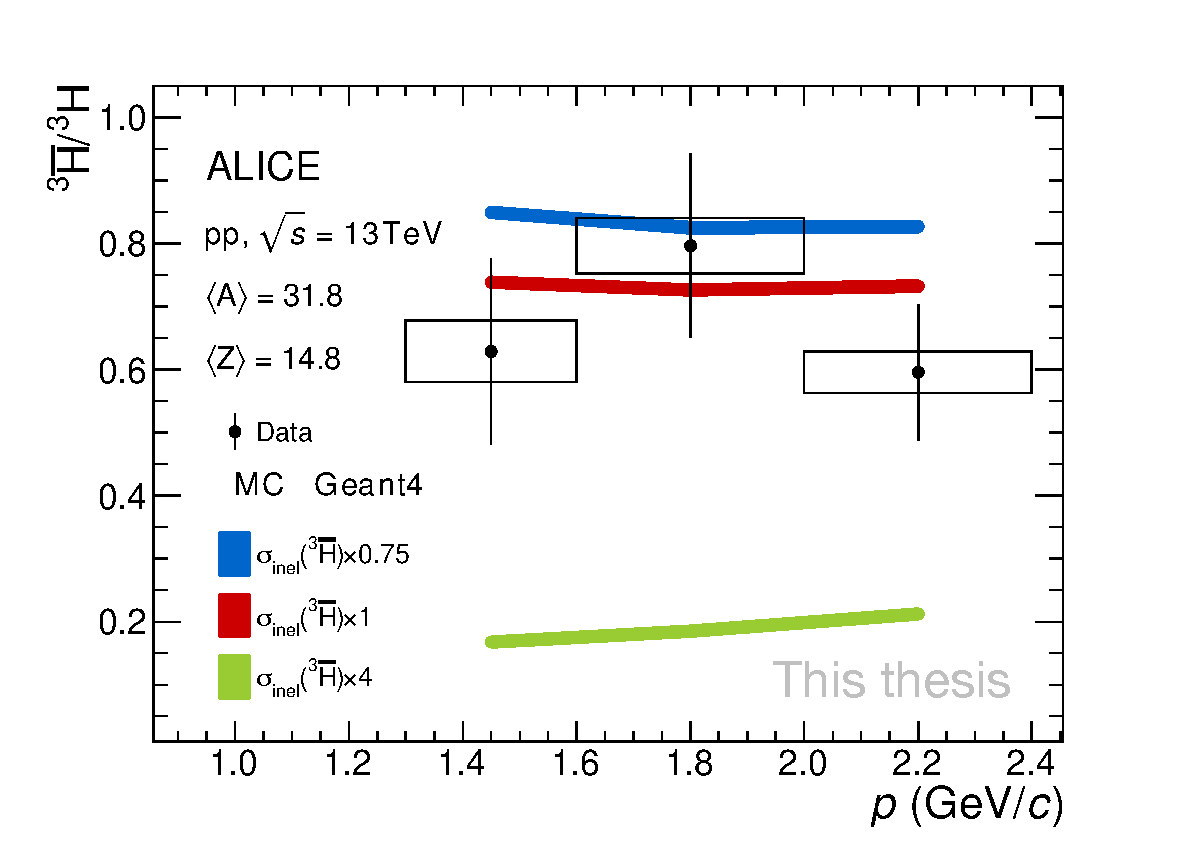
\includegraphics[width=0.48\textwidth]{figures/Anti-triton-to-triton_Ratio.pdf}%pp ratio plot
    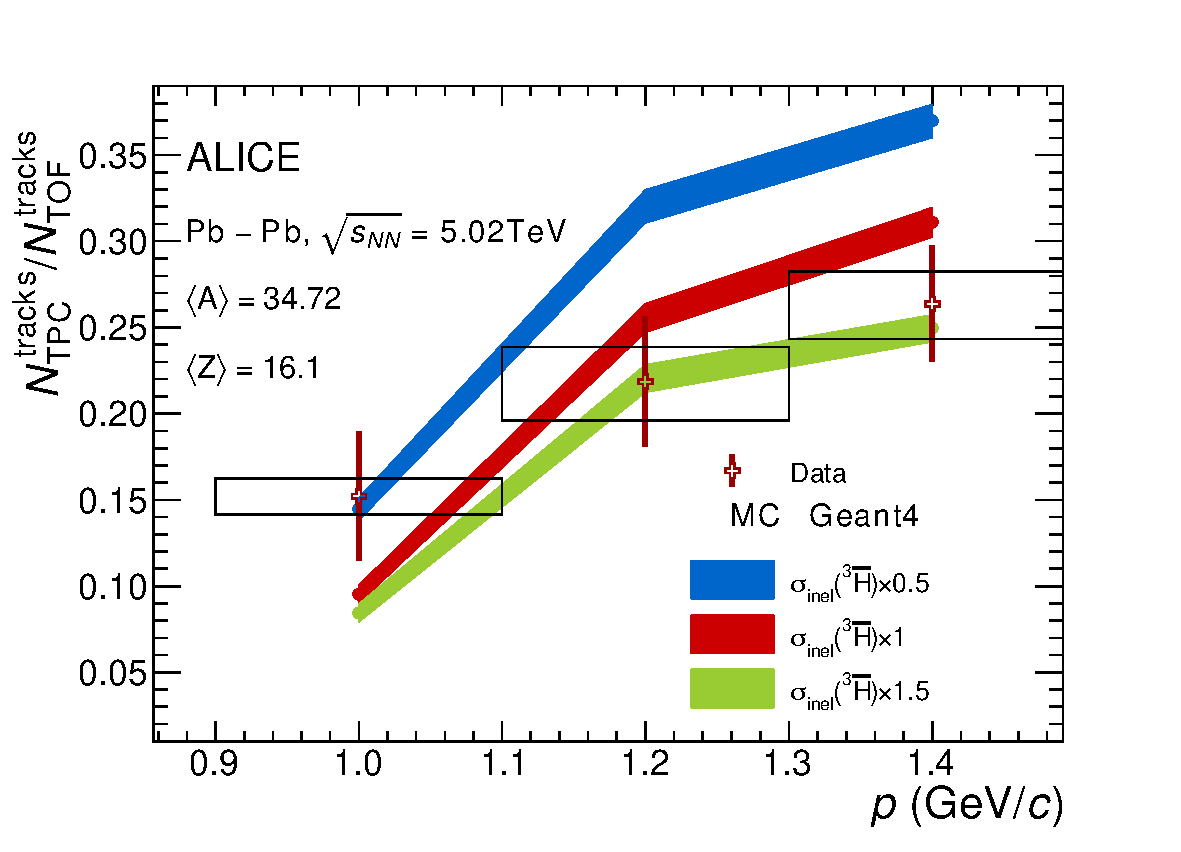
\includegraphics[width=0.48\textwidth]{figures/Anti-triton-TPC-TOF_Ratio.pdf}%sigma inel in pp
    \caption{(Left) \atrit\ /$^3\mathrm{H}$ ratio as a function of momentum, with statistical uncertainties as bars and systematic uncertainties as boxes. The colored lines represent Monte Carlo simulations with varied inelastic cross sections. (Right) \atrit\ TOF-to-TPC ratio as a function of momentum, with statistical uncertainties as bars and systematic uncertainties as boxes. The colored lines represent Monte Carlo simulations with varied inelastic cross sections. }
    \label{fig:Results:tbar:ratios}
\end{figure}

\begin{figure}
    \centering
    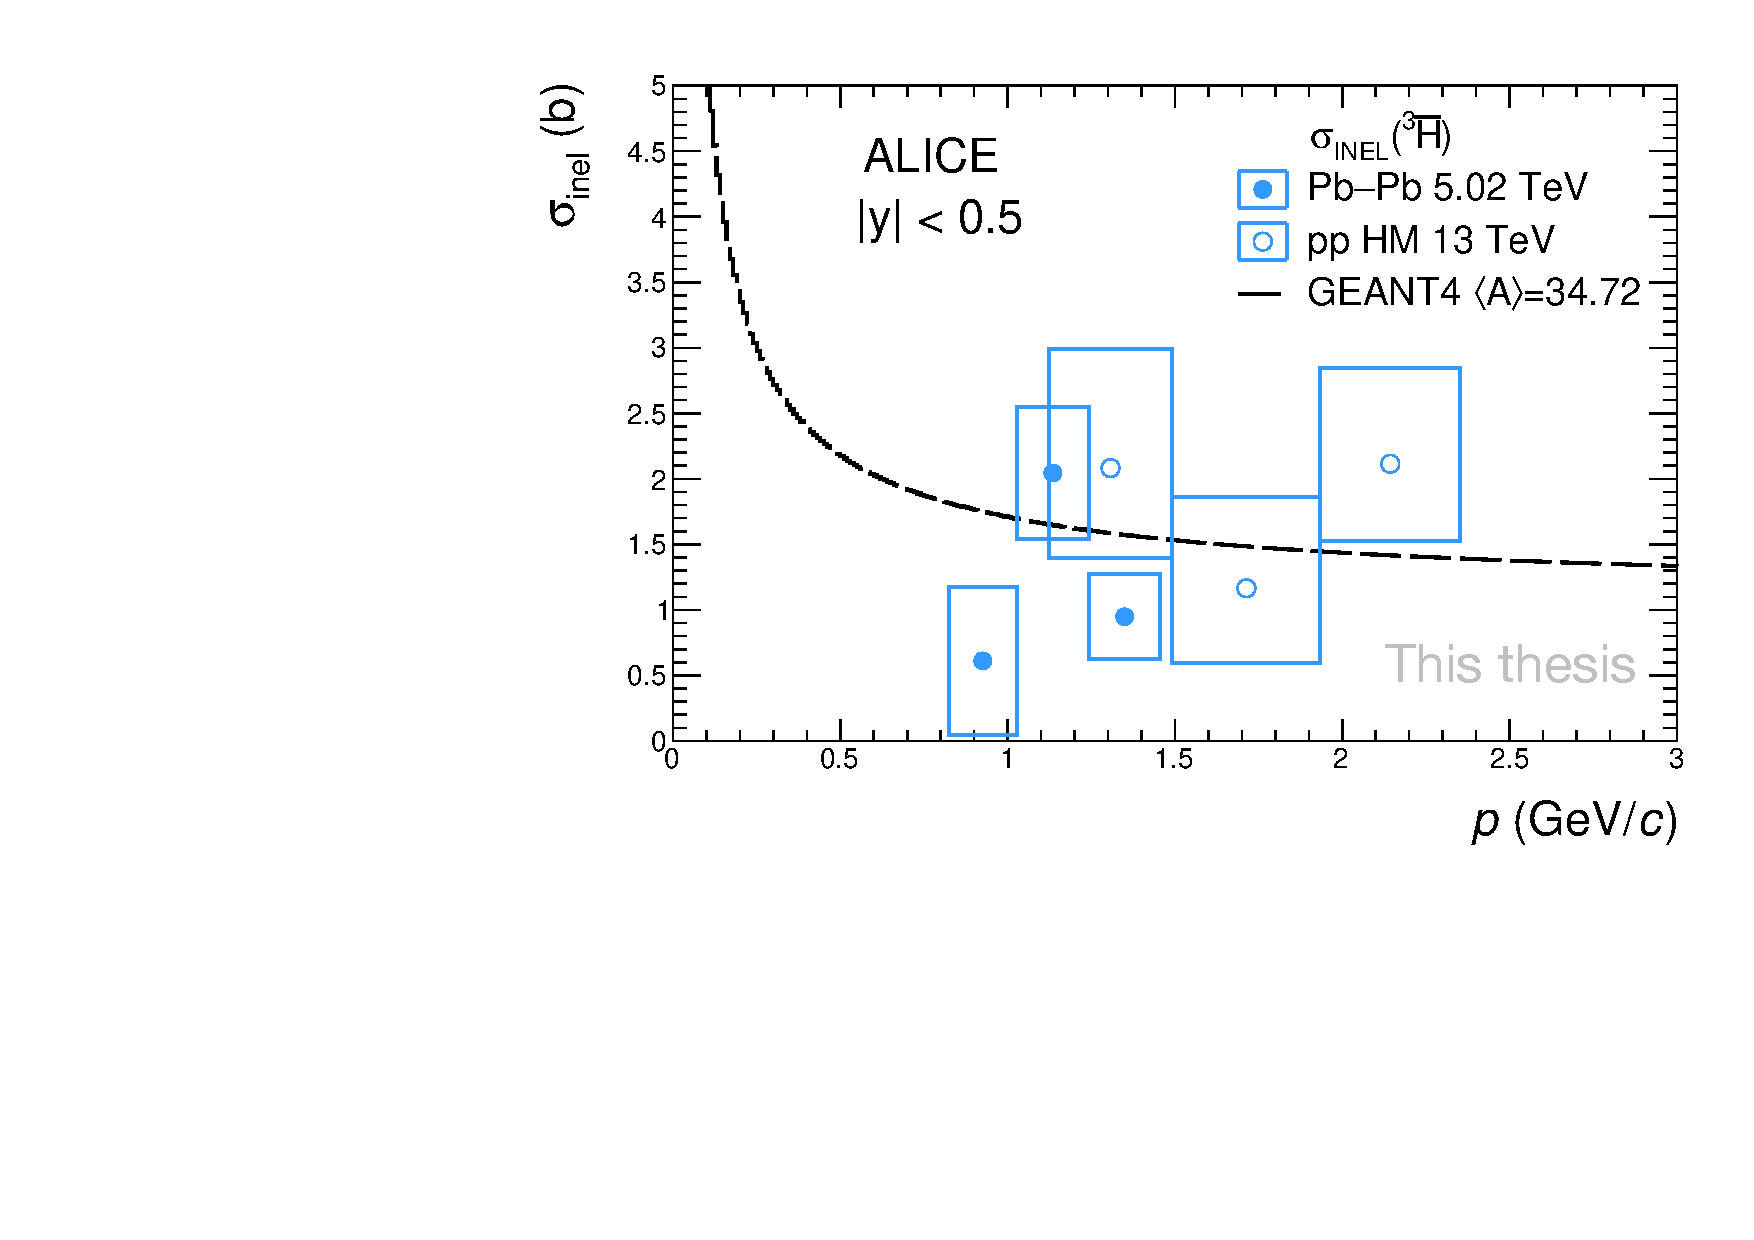
\includegraphics[width=0.48\textwidth]{figures/FinalXS_antit_paper.pdf}%PbPb ratio plot
    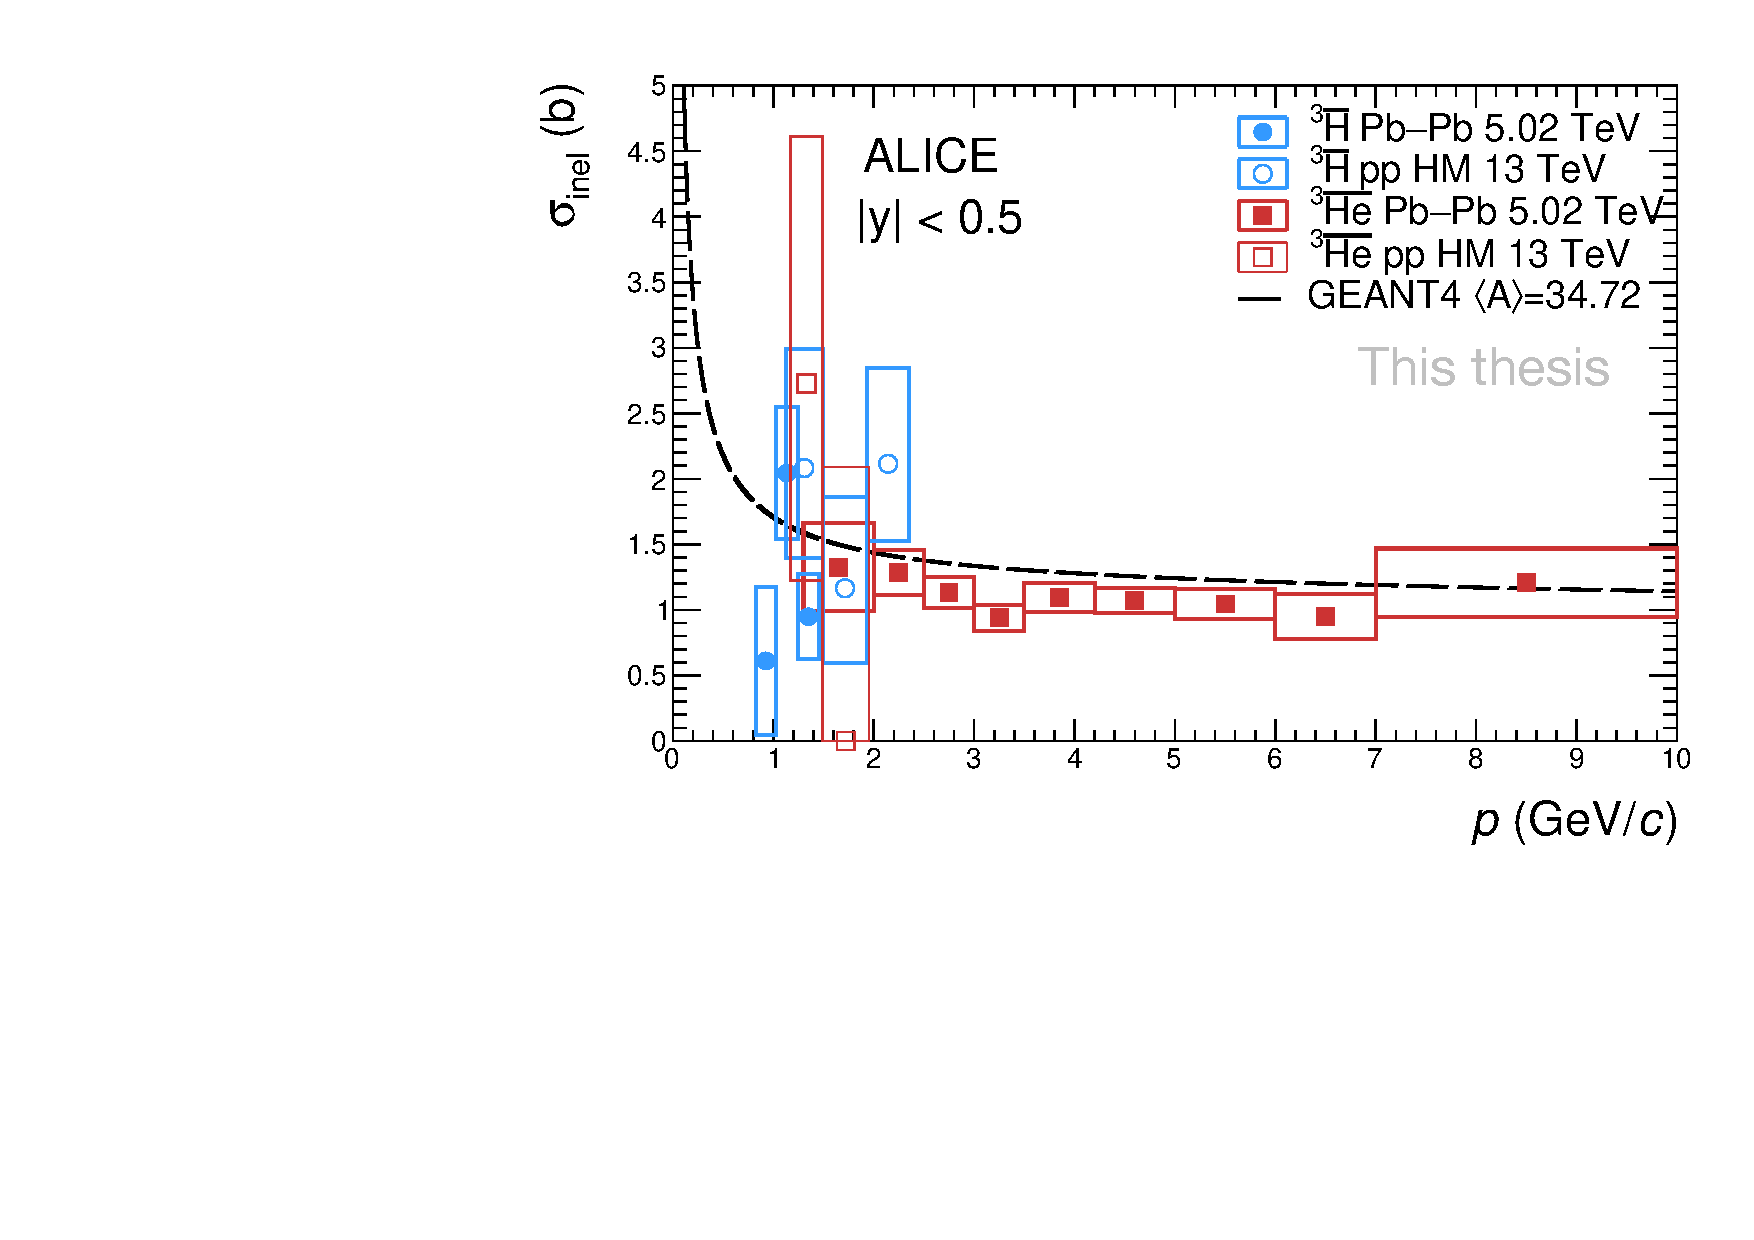
\includegraphics[width=0.48\textwidth]{figures/FinalXS_antitantiHe3_paper.pdf}%sigma inel PbPb
    \caption{(Left) the resulting measurement of \sigmainelH\ using the antibaryon-to-baryon method ($\mathrm{\overline{B}}/\mathrm{B}$) and the TOF-to-TPC method, on the average ALICE material. The colored boxes show the total uncertainty (stat$^2 +$ syst.$^2$). The line shows the parameterization as used in Geant4. (Right) comparison of the \sigmainel\ and \sigmainelH\ measurements.}
    \label{fig:Results:tbar:xs}
\end{figure}


\newpage



